\chapter{Fundamentação Teórica}\label{chp:FUNDAMENTACAO_TEORICA}

Esse capítulo tem como objetivo promover um esclarecimento sobre o arcabouço teórico necessário para o entendimento do trabalho. Como dito anteriormente, assim como diversos outros problemas hoje em dia, a Detecção de Anomalia é resolvida através de técnicas de aprendizado de máquina. Nesse capítulo, será tratado com mais detalhes o que é aprendizado de máquina, e algumas técnicas utilizadas para fazer com que uma máquina aprenda determinada tarefa. Posteriormente, será abordado com mais detalhes como essas técnicas são aplicadas para o contexto específico de Detecção de Anomalia e alguns desafios encontrados nessa aplicação.

% abordados alguns desafios na utilização dessas técnicas para o contexto específico de Detecção de Anomalia especificamente
% á tratado como ué possível que problema de Detecção de Anomalia é resolvido utilizando técnicas de aprendizado de máquina.  tratando-o com mais detalhes e explicando suas motivações e desafios. Será abordado o tema Aprendizado de Máquina, primordial para o entendimento do problema, e seus diversos tipos. E, por último, Redes Neurais, que geralmente é a técnica de aprendizado de máquina utiliza para a identificação de cenários anômalos.

\section{Aprendizado de Máquina}
Aprendizado de Máquina é um subcampo da Inteligência Artificial destinado a fazer máquinas aprenderem tarefas sem serem explicitamente programadas para tal. A área de Aprendizado de Máquina é inspirada por diversas outras áreas, como ciências cognitivas, ciência da computação, estatística, complexidade computacional, teoria da informação, teoria de controle, filosofia e biologia. \cite{machine_learning_yao_liu}

Segundo \citeonline{naqa_e_murphy}, um algoritmo de aprendizagem de máquina é um processo que usa dados como entrada para realizar uma tarefa desejada, sem ser literalmente programado para produzir uma saída em específico, mas se alterando e adaptando sua arquitetura através da experiência, o que é chamado de aprendizado.

Um dos pioneiros na área de Machine Learning foi Arthur Samuel. Em 1959, ele publicou um artigo dissertando sobre um algoritmo que aprendia a jogar Xadrez, afirmando que o aprendizado acontecia entre 8 e 10 horas, e que o computador era capaz de jogar melhor do que a própria pessoa que o programou. \cite{arthur_samuel_xadrez}

Posteriormente, outro grande nome da área de \ac{ML}
, Tom M. Mitchell, professor universitário, fundador e ex-presidente do Departamento de Machine Learning da Universidade
Carnegie Mellonara, definiu aprendizado de máquina da seguinte forma: \textit{"Pode-se dizer que um programa de computador aprende a partir da experiência E, a executar alguma classe de tarefas T, dada uma medida de desempenho P, quando sua performance nas tarefas em T, medida por P, melhora com a experiência E."}\cite{machine_learning_tom_mitchell}

Como dito anteriormente, o processo de aprendizagem de máquina requer dados como entrada. E nas últimas décadas, devido ao \textit{boom} dos dados, onde a quantidade de informações geradas por pessoa cresce a cada ano, essa área vem se disseminando muito rapidamente. Grande exemplo disso é o \href{https://openai.com/blog/chatgpt}{\textit{ChatGPT}}, um \textit{bot} lançado pela empresa de IA, OpenAI, em 2022, que é livre para qualquer usuário da internet testar.

% TO DO : encontrar artigo q embase a parte dos "dados gerados por pessoa crescerem muito". Só achei esse link na internet: https://uoledtech.com.br/blog/transformacao-digital-e-so-tecnologia

%comments saved

\section{Tipos de Aprendizado de Máquina}

A ciência de fazer máquinas aprenderem é dividida em três grandes tipos: aprendizado supervisionado, aprendizado não-supervisionado e aprendizado por reforço.

No aprendizado supervisionado, os dados utilizados são rotulados, isto é, além das características dos dados, tem-se também a resposta esperada que a máquina forneça para cada ocorrência do dado. Assim, a ideia é que o algoritmo vá aprendendo ao longo do treinamento as características mais importantes e os padrões gerais existentes nos dados, a fim de generalizar o suficiente para prever as respostas corretas para exemplos de dados ainda não vistos.

Nesse tipo de aprendizado, existem as tarefas de classificação e de regressão. [REF] Uma tarefa é dita de regressão, quando o rótulo dos dados é contínuo, está no conjunto dos Reais. Ao passo que, uma tarefa é dita de classificação, quando o domínio dos rótulos dos dados é um subconjunto bem definido de valores, geralmente inteiros, onde cada valor especifica uma classe.

Enquanto o aprendizado supervisionado utiliza dados rotulados, no aprendizado não supervisionado, os dados não possuem rótulos ou gabaritos. Nesse modelo, o que ocorre é uma aprendizagem heurística no decorrer do treinamento.

% falar um pouco mais sobre o não supervisionado %

Há, ainda, entre o aprendizado supervisionado e o não-supervisionado, o semi-supervisionado, que consiste numa tentativa de suprir as desvantagens de cada um dos métodos com as vantagens do outro. Nessa abordagem, o treinamento começa com os dados obtidos que possuam rótulo, a fim de adquirir algum conhecimento a respeito do problema que ajude no aprendizado com os dados não rotulados, que se segue.\cite{tcc_anomalia_2020}

Além do aprendizado com supervisão ou não, existe ainda um outro tipo de aprendizado, que começou a surgir na literatura na década de 1990, o aprendizado por reforço. No ano de 1998, \citeauthor{drive_a_bicycle_rl_jette} publicaram um artigo explicando como seria possível aprender a andar de bicicleta utilizando aprendizado por reforço. No mesmo ano, \citeauthor{rl_an_introduction} publicaram o livro \textit{Reinforcement Learning: An Introduction}, explicando mais em detalhes o aprendizado por reforço. \cite{rl_an_introduction}

Esse tipo de aprendizado se baseia fundamentalmente na interação com o ambiente, onde, a cada iteração, a máquina capta as percepções do estado do ambiente e realiza alguma ação. E essas ações são medidas como boas ou não através de uma função chamada recompensa ou penalização.

Tendo dado uma breve introdução a respeito dos diversos tipos de aprendizado de máquina, serão explicados a seguir conceitos mais específicos necessários para o entendimento do trabalho aqui proposto, bem como para o desenvolvimento da solução de Detecção de Anomalia.


% DRAFT --- DRAFT --- DRAFT 
% No aprendizado supervisionado, para medir o aprendizado, temos uma função que, de algum modo, calcula a diferença entre os rótulos esperados (reais) e os obtidos como saída do algoritmo no conjunto de teste.

% é dito que a tarefa é de regressão. Enquanto, quando o rótulo está num conjunto bem definido 
% Nesse tipo de aprendizado, para medir o aprendizado, utiliza-se uma função, f : X X Y -> R. é necessária uma medida para saber

% comments saved

% lero-lero o q aprendizado ?
% tipos de aprendizado
% supervisionado def
% supervisionado fç de custo / performance
% não supervisionaod def (exemplo)
% semi-supervisionado def
% por ref def
% por ref mais deta (agente, tempo, função)


\section{Redes Neurais Artificiais}
Um dos modelos de \ac{IA} mais famosos e que tem sido muito utilizado hoje em dia é o de Redes Neurais Artificias (\textit{Artificial Neural Networks} ou \textit{ANNs}). Isso se dá devido ao fato de que, com esse modelo, é possível o aprendizado de muitos problemas complexos, que outros modelos não são capazes de aprender. Alguns desses problemas são o reconhecimento de fala, reconhecimento facial, reconhecimento de caracter escrito a mão, classificação de imagens, detecção de objetos em imagens, entre outros.

O modelo de \ac{ANN} foi inspirado nas redes neurais biológicas existentes nos seres vivos. De forma simplória, é possível defini-lo como um conjunto de unidades simples, densamente interconectadas, onde cada unidade recebe um número de entrada real, que pode ser a saída de outras unidades, e produz um único valor de saída real, que pode se tornar a entrada de outras unidades.\cite{machine_learning_tom_mitchell, tcc_anomalia_2021}
% TO DO : how to deal with 2 references?

\subsection{Perceptron}
A forma mais simples de unidade de rede neural que existe na literatura é o \textit{perceptron}. O \textit{perceptron} foi criado por \citeauthor{perceptron_frank_rosenblatt}, psicólogo americano, em 1958, e nada mais é do que um algoritmo iterativo que produz um resultado através da
combinação linear entre os valores de entrada \(x_{1}, x_{2}, x_{3}, ..., x_{n}\) e um vetor de valores
\(w_{0}, w_{1}, w_{2}, ..., w_{n}\) que serão otimizados durante a execução.\cite{perceptron_frank_rosenblatt}\cite{tcc_anomalia_2020}
% TO DO : how to deal with 2 references?

O vetor \(\overrightarrow{w}\), chamado de vetor de pesos, é composto de valores reais, onde cada \(w_{i}\) determina a contribuição da entrada \(x_{i}\) à saída do perceptron.\cite{machine_learning_tom_mitchell} Caso o resultado da combinaçao linear entre os vetores seja maior do que 0, a saída do perceptron é 1, se não, é -1. Assim, a função \(\ \theta (x_{1}, ..., x_{n})\) computada pelo \textit{perceptron} é definida da seguinte forma:
\begin{equation}
%\[
    \theta (x_{1}, \cdots, x_{n}) = 
    \begin{cases}
         \quad1       & \quad \text{caso } w_{0} + w_{1}x_{1} + ... + w_{n}x_{n} > 0\\
        -1  & \quad \text{caso contrário}
    \end{cases}
%\]
\label{eq:eq_perceptron_extenso}
\end{equation}

Ainda, para simplificar, podemos imaginar uma entrada constante \(x_{0} = 1\). Dessa forma, temos \( \sum_{i=0}^n w_{i}x_{i} \), que também pode ser chamado de produto escalar entre \(\overrightarrow{w}\) e \(\overrightarrow{x}\). Sendo assim, a \refequation{eq:eq_perceptron_extenso} também pode ser descrita como:
\begin{equation}
%\[
    \theta (x_{1}, \cdots, x_{n}) = sign(\overrightarrow{w}.\overrightarrow{x})
%\]
\label{eq:eq_perceptron_com_sign}
\end{equation}
onde
\begin{equation}
%\[
    sign (z) = 
    \begin{cases}
         \quad1       & \quad \text{caso } z > 0\\
        -1  & \quad \text{caso contrário}
    \end{cases}
%\]
\label{eq:eq_perceptron_sign}
\end{equation}

Vale ressaltar que a função \textit{sign}, no contexto de Redes Neurais, pode também ser chamada de função de ativação, como será explicado com mais detalhes nos próximos tópicos do trabalho.

% Ainda, para simplificar, podemos imaginar uma entrada constante \(x_{0} = 1\). Dessa forma, temos que \( \theta (x_{1}, \cdots, x_{n}) \), pode ser definida como:
% \begin{equation}
% %\[
%     \theta (x_{1}, \cdots, x_{n}) = \sum_{i=0}^n w_{i}x_{i} > 0
% %\]
% \label{eq:eq_perceptron_somatorio}
% \end{equation}



O processo de aprendizagem no algoritmo \textit{perceptron} pressupoe um conjunto de dados com suas classificações (aprendizado supervisionado), e ocorre da seguinte forma: o vetor de pesos, \(\overrightarrow{w}\), é iniciado com valores arbitrários, e esses valores são atualizados sempre que algum exemplo de dado fornecido for classificado erroneamente. Após um número finito de iterações, o algoritmo encontra os valores para os parâmetros (pesos) que permite obter os melhores resultados. \cite{neural_network_learning_anthony_bartlett} \cite{tcc_anomalia_2020}
% TO DO : how to deal with 2 references?

A fórmula de atualização dos pesos é dada por:
\begin{equation}
%\[
    w_{i} = w_{i} + \eta y_{i}x_{i}
%\]
    \label{eq:eq_perceptron_atualizacao_pesos}
\end{equation}

onde \(\eta\) é a taxa de aprendizado, uma constante positiva que regula o quanto os pesos são alterados a cada passo do algoritmo, e \(y_{i}\) corresponde a um elemento do vetor \(\overrightarrow{y}\), que contém as classificações (alvos) dos dados.

Apesar da enorme importância e entusiasmo na época com o \textit{perceptron}, anos mais tarde, em 1969, os pesquisadores \citeauthor{perceptron_not_linear_separable_marvin_seymour} observaram que o modelo não era capaz de resolver problemas não linearmente separáveis, como a simples função booleana XOR. Contudo, uma nova alternativa é proposta por \citeauthor{mlp_gradient_descend_paul} em 1975: o \textit{perceptron} multicamada (\textit{multilayer perceptron} ou MLP).


% PAREI AQUI
% numeração das fórmulas ?
% mencionar fç sign como fç de ativação lá em cima
% baixar e publicar code do TCC atualizado no final


\subsection{Multilayer Perceptron}

O \ac{MLP} nada mais é do que um conjunto de \textit{perceptrons} interconectados (nota-se que aqui, começamos a perceber o sentido de \textbf{redes} neurais). Uma \ac{MLP} é organizada em camadas, que é simplesmente um conjunto de neurônios em sequência, e a saída de uma camada é a entrada para outra. Além disso, uma \ac{MLP} deve ter, pelo menos uma camada oculta, que fica entre a camada de entrada e a camada de saída.

\begin{figure}[h] %[!] --> latex escolhe melhor posição [h] --> posição exata em q definimos a img "here" [t] --> topo  [b] --> bottom [p] --> vai p uma pág sozinha
  \centering
  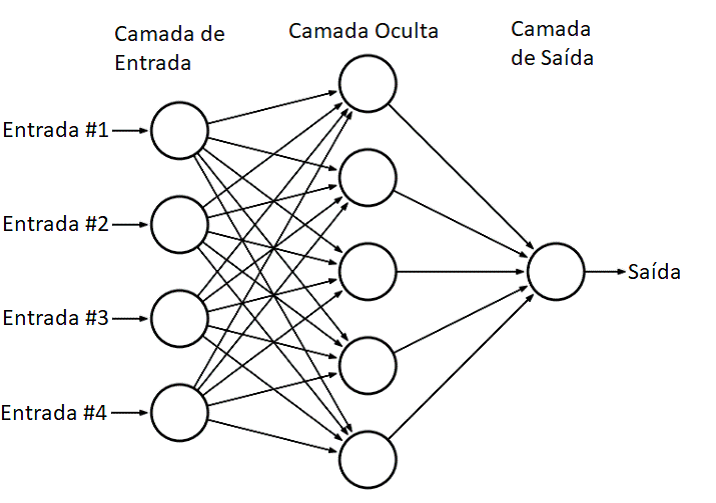
\includegraphics[width=0.6\textwidth]{imagens/arquitetura_mlp.png}
  \caption{Arquitetura MLP. Imagem adaptada de \cite{mlp_architeture_hassan}. \cite{tcc_anomalia_2021}}
  \label{fig:arquitetura_mlp}
  %\legend{Fonte: o autor.}
\end{figure}

A razão pela qual a rede \ac{MLP} resolve o problema do não aprendizado de funções não linearmente separáveis do \textit{perceptron} é a função utilizada nos neurônios. No modelo \textit{perceptron}, tínhamos a função \textit{sign}, que determinava um limiar para a saída ser 1 ou -1. No caso do \ac{MLP}, utiliza-se funções não lineares como função de ativação. E, a conexão de vários \textit{perceptrons} em rede utilizando funções não lineares para o aprendizado é justamente o que possibilita que se aprenda funções não lineares e extremamente complexas. \cite{MLP_gardner}

%%%%%%%%%%%%%%%%%%%%%%%%%%%%%%%%%%%%%%%%%%%%%%
% O que é MLP(CONJ DE PERCEPTRONs conectados, q permitem resolver a limitação do perceptron)
% img arquitetura
% conj d funções não lineares com fç de ativação permite aprender qq parada

\subsection{Função de Ativação}
Como já mencionado anteriormente, a função de ativação consiste em uma das partes da computação do neurônio (ou \textit{perceptron}). A primeira parte é a soma da multiplicação dos dados recebidos com os pesos do neurônio, que então é fornecida como entrada para a função de ativação, que determina a saída do neurônio, consistindo na segunda parte da computação.

Como a maioria dos problemas do mundo real possuem características não lineares, funções de ativação não lineares são preferíveis ao invés de funções lineares.\cite{activation_functions_ann_sharma}. Esse também é o motivo pelo qual funções de ativação são necessárias, já que sem elas, as redes neurais teriam sempre saídas lineares, e agiriam apenas como modelos de regressão linear com desempenho limitado.\cite{tcc_anomalia_2021}

%%%%%%%%%%%%%%%%%%%%%%%%%%%%%%%%%%%%%%%%%%%%%%
% intro opcional sobre oq é a fç de ativação
% Sharma e Athaiya : pq fçs não lineares são necessáriase importantes (2021)
% explicar sigmoid, com fórmula, gráfico. E sua desvantagens
% explicar tanh, com  fórmula, gráfico. E suas desvantagens
% explicar ReLu, com  fórmula, gráfico. E suas desvantagens
% explicar suscintamente LeakyRelu e Parametric ReLu



\subsection{Back Propagation}



\section{Redes Neurais Convolucionais}

\section{Autoencoder}

\section{Classificador}

\begin{comment}
Esse capítulo será responsável por dar uma base teórica a proposta. 
A ideia é que o leitor, com um breve conhecimento prévio, tenha a capacidade de ler esse material e consiga ter a capacidade de entender tecnicamente a proposta do projeto final.
Dependendo do assunto, poderá ter mais de uma área de resumo, podendo ficar cada uma em uma seção ou serem capítulos separados.

No caso de um único capítulo, deverá ter um breve resumo antes de iniciar a seção explicando o que este capítulo fará. Caso seja capítulo separado, poderá introduzir a área diretamente sem a criação de uma seção ou criar uma seção chamada "Introdução" e o nome do capítulo pode ser o nome da área.
\end{comment}